\documentclass[a4:paper,14pt]{article}
\usepackage{graphicx}
\usepackage{sectsty}
\usepackage{array}
\usepackage{amsthm}
\usepackage{titlesec}
\usepackage{indentfirst}
\usepackage{xr}
\usepackage{subfigure}
\usepackage[round, sort, numbers]{natbib}
\usepackage{url}
\usepackage{setspace}
\usepackage{pdfpages}
\usepackage{amsmath}

\setcitestyle{square}
\graphicspath{{images/}}

\allsectionsfont{\centering}

\makeatletter
\makeatother

\usepackage{geometry}
\geometry{left=2.5cm}
\geometry{right=1.5cm}
\geometry{top=2cm}
\geometry{bottom=2cm}

\newcommand{\norm}[1]{\left\lVert#1\right\rVert}
\newcommand{\isum}[2][j]{\sum \limits_{#1=1}^{\infty}{#2}}
\newcommand{\operator}[1]{\mathcal{R}{#1}}
\newcommand{\supp}{\mathop{\mathrm{supp}}}
\newtheorem{remark}{Замечание}


\begin{document}

shock-like profiles

\begin{equation}\label{shock_like}
  U(x) = -2\sigma\tanh{(\sigma(x - \frac{1}{2}))},
\end{equation}

where $\sigma \ge 0$.



\begin{figure}[h]
  \centering
  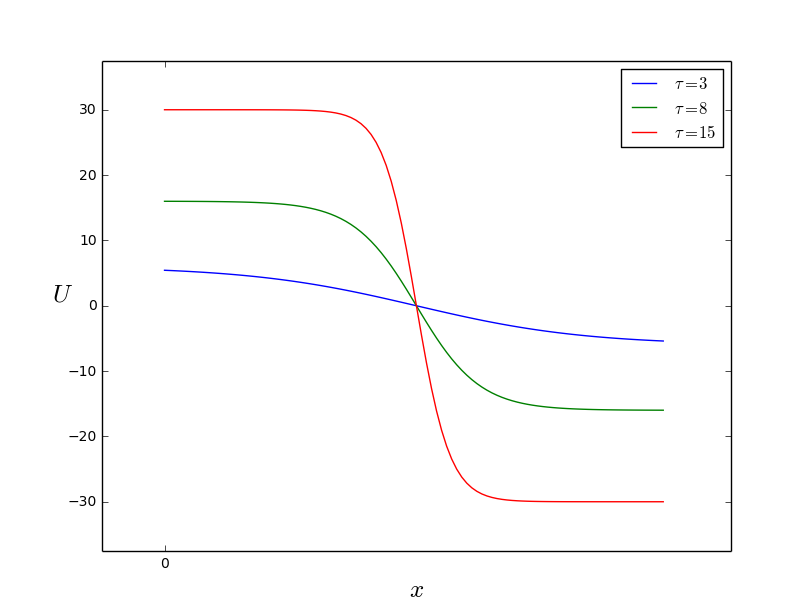
\includegraphics[width=4in]{fig1}
  \caption{$U(x)$}
\end{figure}

Transformation: 

\begin{equation}
  G(x) = \frac{\cosh(\sigma(x - \frac{1}{2}))}{\cosh(\frac{\sigma}{2})}
\end{equation}

\begin{figure}[h]
  \centering
  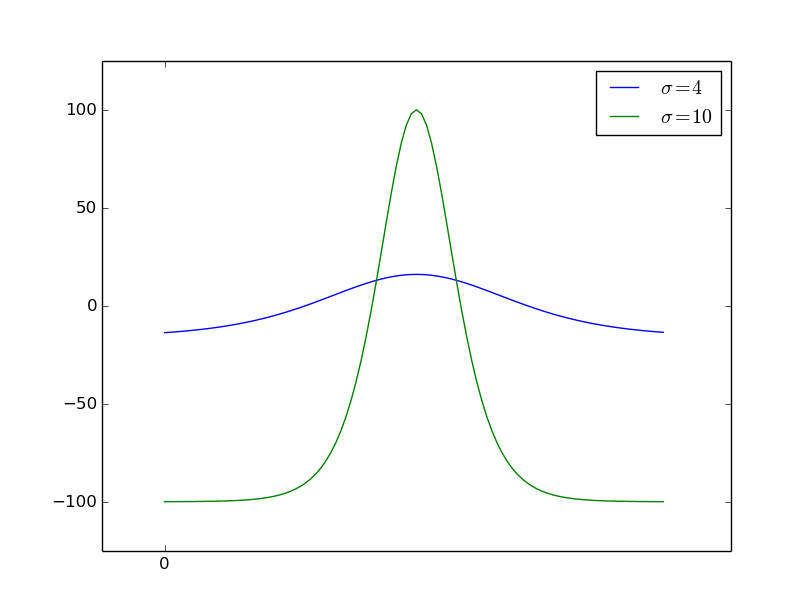
\includegraphics[width=4in]{fig2}
  \caption{$\sigma^2 \left( \frac{2}{\cosh^2(\sigma(x - \frac{1}{2}))} - 1 \right)$}
\end{figure}


\begin{gather}
    \theta_0 = \frac{\sin(\pi x)}{G(x)} \\*
    \sigma = 3
\end{gather}


\begin{figure}[h]
\centering
\begin{minipage}{.5\textwidth}
  \centering
  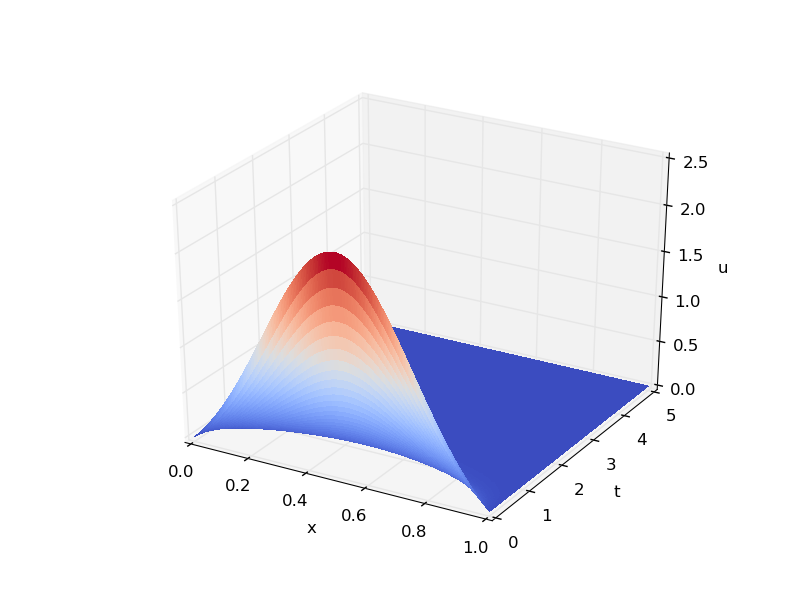
\includegraphics[width=3.5in]{ex_s3}
  \caption{Uncontrolled}
  \label{fig:test1}
\end{minipage}%
\begin{minipage}{.5\textwidth}
  \centering
  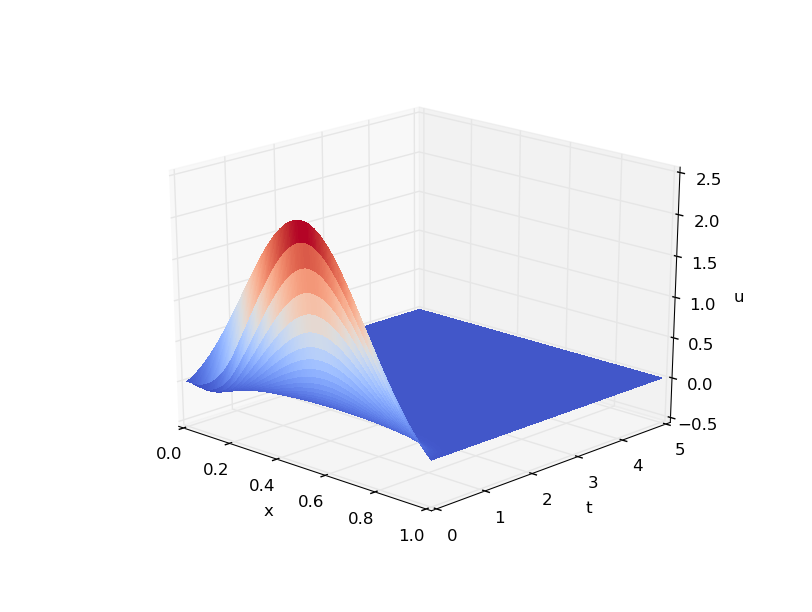
\includegraphics[width=3.5in]{re_s3}
  \caption{Control $m = 2, \; r = 15$}
  \label{fig:test2}
\end{minipage}
\end{figure}



\begin{gather}
    \theta_0 = \frac{\sin(\pi x)}{G(x)} \\*
    \sigma = 15 \\*
    \omega = (0, 0.2), \; r = 15, \; m = 2
\end{gather}


\begin{figure}[h]
\centering
\begin{minipage}{.5\textwidth}
  \centering
  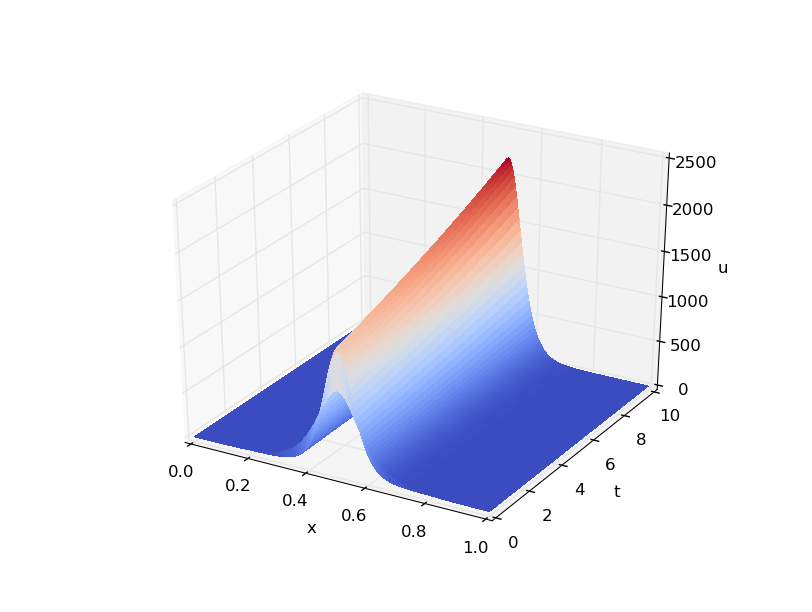
\includegraphics[width=3.5in]{ex_s15}
  \caption{Uncontrolled}
  \label{fig:test1}
\end{minipage}%
\begin{minipage}{.5\textwidth}
  \centering
  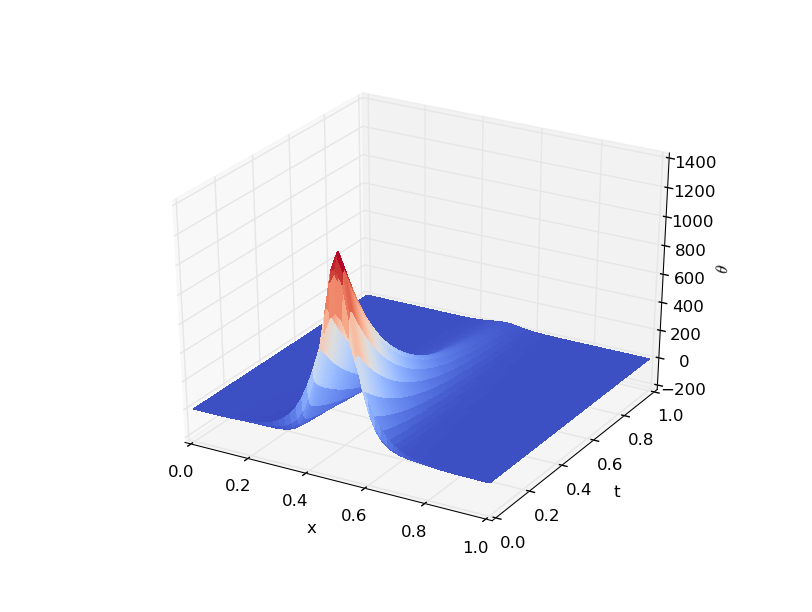
\includegraphics[width=3.5in]{re_s15}
  \caption{Control $m = 2, \; r = 15$}
  \label{fig:test2}
\end{minipage}
\end{figure}

\begin{gather}
    \theta_0 = \frac{\sin(10 \pi x)}{G(x)} \\*
    \sigma = 15 \\*
    \omega = (0, 0.2), \; r = 15, \; m = 2
\end{gather}



\begin{figure}[h]
\centering
\begin{minipage}{.5\textwidth}
  \centering
  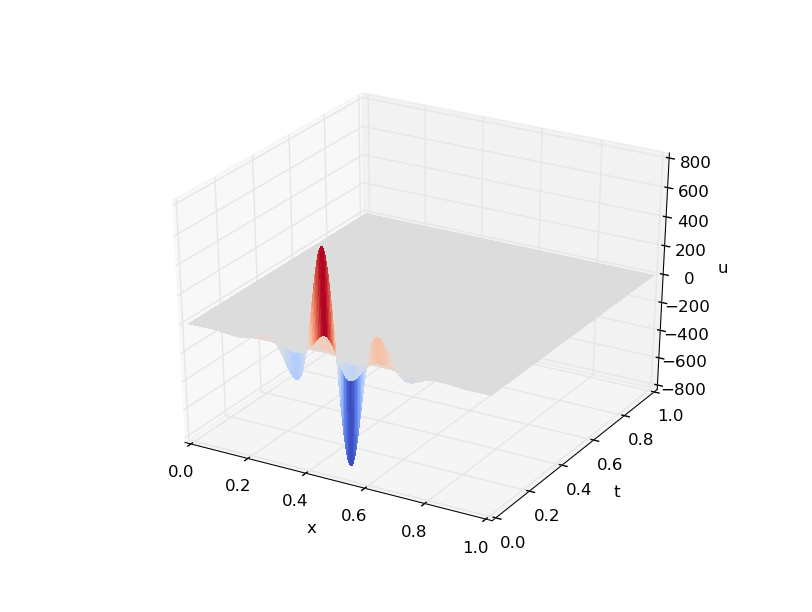
\includegraphics[width=3.5in]{ex_sin10_s15}
  \caption{Uncontrolled}
  \label{fig:test1}
\end{minipage}%
\begin{minipage}{.5\textwidth}
  \centering
  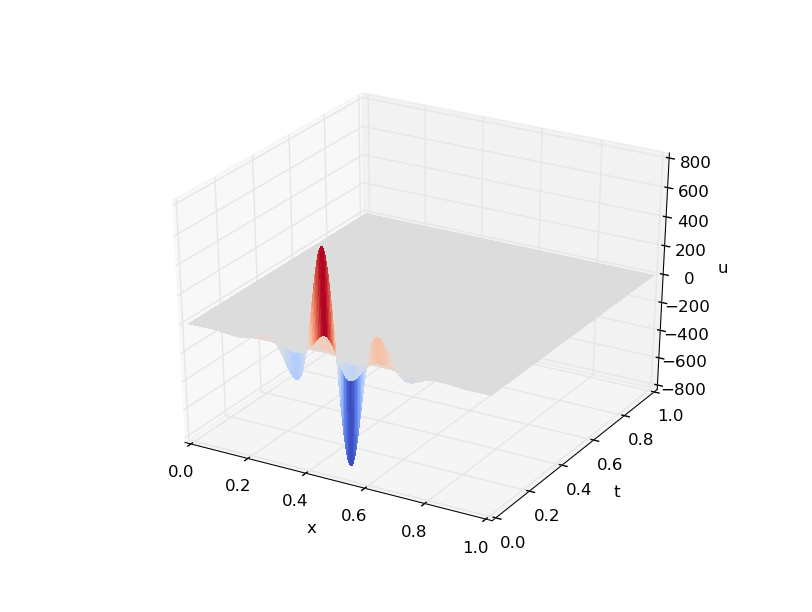
\includegraphics[width=3.5in]{re_sin10_s15}
  \caption{Control $m = 2, \; r = 15$}
  \label{fig:test2}
\end{minipage}
\end{figure}

\begin{gather}
    \theta_0 = \frac{x^2}{G(x)} \\*
    \sigma = 15 \\*
    \omega = (0, 0.2), \; r = 15, \; m = 2
\end{gather}

\begin{figure}[h]
\centering
\begin{minipage}{.5\textwidth}
  \centering
  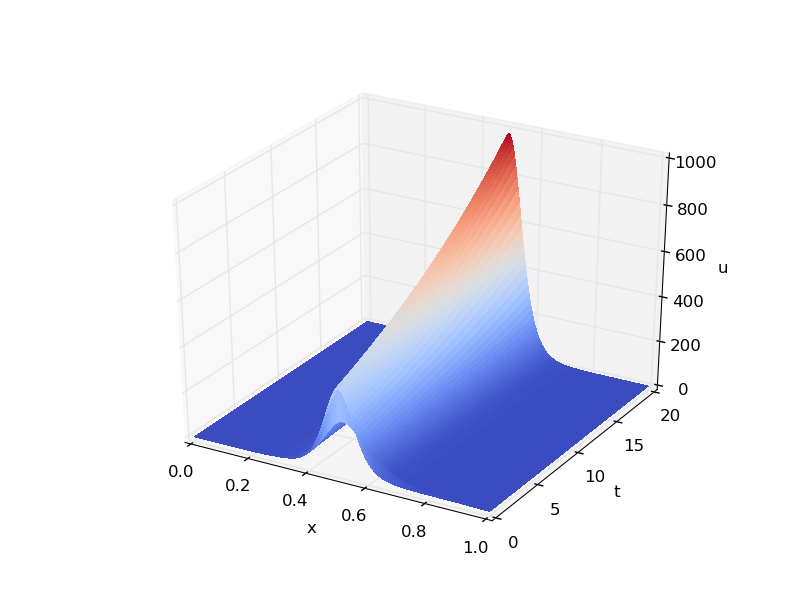
\includegraphics[width=3.5in]{ex_x2_s15}
  \caption{Uncontrolled}
  \label{fig:test1}
\end{minipage}%
\begin{minipage}{.5\textwidth}
  \centering
  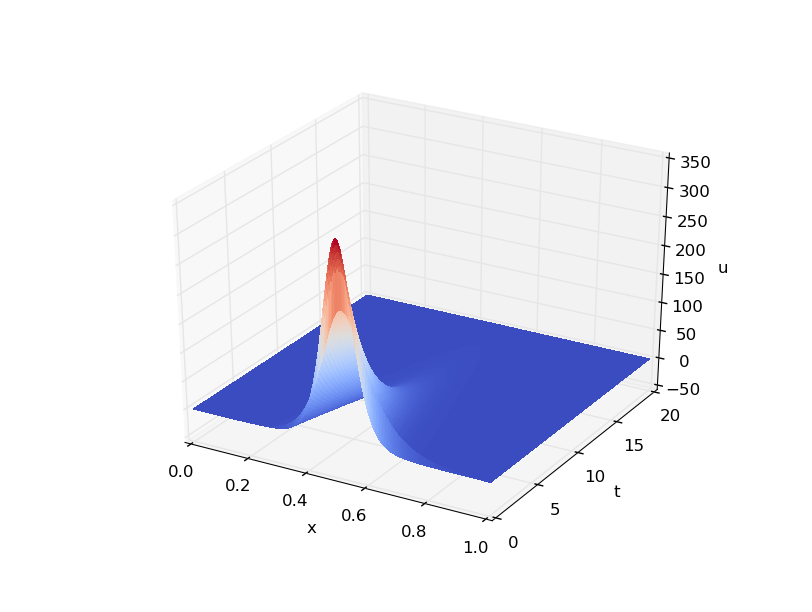
\includegraphics[width=3.5in]{re_x2_s15}
  \caption{$\omega = (0, 0.2), \; r = 15, \; m = 2$}
  \label{fig:test2}
\end{minipage}
\end{figure}


\end{document}
